\chapter{Gas Electron Multiplier} % (fold)
\label{cha:gas_electron_multiplier}

Gas Electron Multiplier (GEM) is a new idea from Fabio Sauli at CERN \cite{Sauli1997}. Developed as a way of boosting the performance of microstrip gas chambers. The objective is to match the harsh running conditions of experiments at CERN's LHC collider, where detectors will have to cope with high data rates and will be exposed to intense bombardment by high-energy particles \cite{detector:1732870}.

GEM is a thin sheet of plastic coated with metal on both sides and chemically pierced by a regular array of holes a fraction of a millimetre across and apart. Applying a voltage (about 500V on 50$\mu$) across the GEM conducting layers, the resulting high electric field in the holes makes an avalanche of ions and electrons pour through each. The GEM foil is shown in Figure \ref{fig:gem}.

\begin{figure}[!htbp]
	\centering
	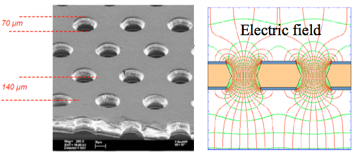
\includegraphics[width=0.95\textwidth]{figures/GEM/KEKDTP3.jpg}
	\caption{(Left) The gas electron multiplier (GEM) foil can image two-dimensional position of particles passing through a gaseous chamber. (Right) The cross sectional view of the GEM shows strong electric fields in the vicinity of holes where electron signals are amplified.}
	\label{fig:gem}
\end{figure}

The region inside GEM detector consists of a drift electrode, a conversion and drift region, a GEM mesh collecting and multiplying the charge in a gas avalanche, and induction gap in which a high electric field is used to extract and drift the electrons towards the collecting electrodes. This is shown in Figure \ref{fig:gemgaps}. The large effective gains (up to $10^4$), full efficiency of detection and very good localization accuracies for minimum ionizing particles is promising to us. In the thin gap of GEM few tens of primary ion pairs creates; cascading to two GEM meshes so it can provide large gains and better performances \cite{Bressan1999}.
\begin{figure}[!htbp]
	\begin{center}
		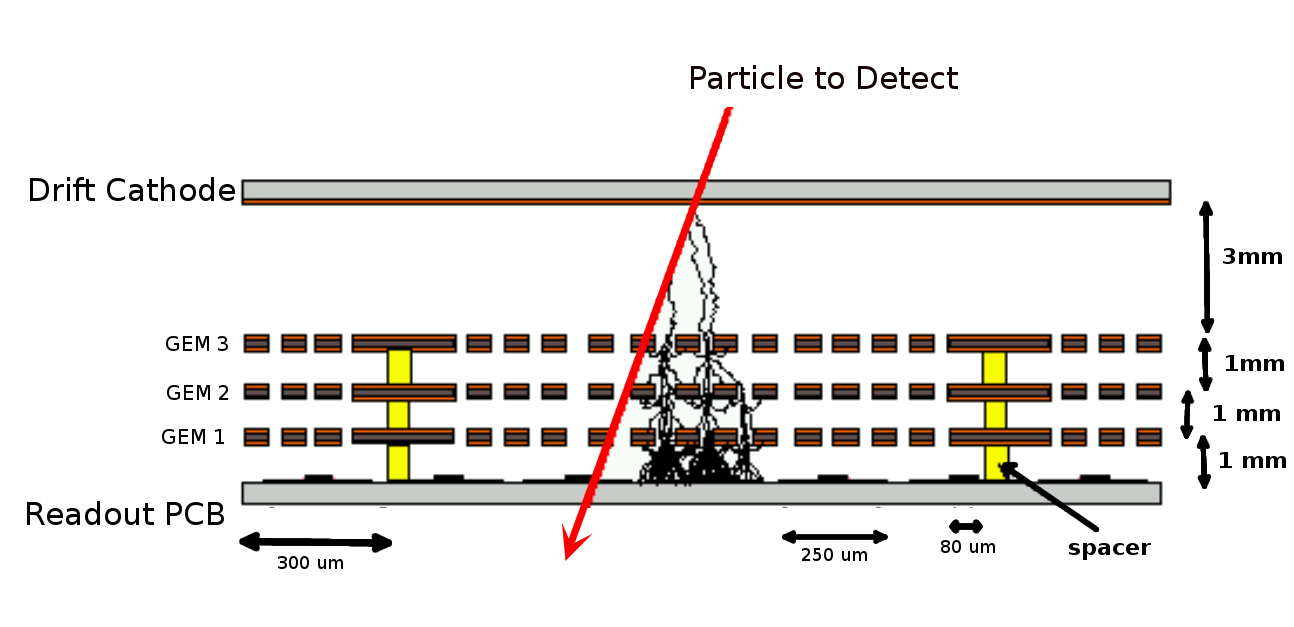
\includegraphics[width=0.95\textwidth]{figures/GEM/triple_gem.png}
		\caption{Illustration of GEM working}
		\label{fig:gemgaps}
	\end{center}
\end{figure} 

\section{GEM for CMS}
The CMS experiment was designed to have a highly redundant muon system using three detector technologies: DT, CSC and RPC. The endcap regions rely on CSC and RPC for $|\eta|<1.6$. For higher $\eta~ (|\eta|>1.6)$ regions, the system has limited redundancy and only CSC are installed. In the future running of LHC at full luminosity, the particle rate in the forward region is expected to reach several tens of kHz/$cm^2$ and the integrated charge will reach several $C/cm^2$, which make the use of the originally planned RPC technology questionable. To overcome these limitations, the CMS GEM collaboration proposed the GEM as a potential candidate to upgrade the high-$\eta$ region of the forward muon system \cite{Colaleo:2021453}. 
%The CMS muon system was designed as a highly hermetic and redundant muon system, composed of three detection technologies. Precision measurements are provided by \gls{dt} in the barrel, covering acceptances up to $|\eta|<1.2$, and \gls{csc} in the endcaps covering $1.0 < |\eta|<2.4$. \gls{rpc} ensures adequate redundancy and triggering up to $\eta | > 1.6$ where the background particle rates are highest and the bending in the magnetic field is smallest.

The chosen technology are GEM, where amplification occurs in the narrow wholes of a thin kapton foil. Three subsequent stages/foils allow for a reasonable amplification at every stage/foil while providing a high total amplification. Two of such triple-GEM chambers are combined to a so called super chamber.

The proposed upgrade targets the following improvements:
	\begin{itemize}
		\item Re-establish the redundancy in the difficult region beyond $\eta = 1.6 $
		\item Improve tracking performance in the high rate environment
		\item The combined operation of CSC and GEM detectors allows a measurement of the bending angle at trigger level, thus strongly reducing the rate of mis-measured muons driving the triggers rate.
	\end{itemize}

\section{Detector Design Description For Test Beam Analysis}
The full design of the GEM chamber is shown in Figure \ref{fig:ge11}.
\begin{figure}[!htbp]
	\begin{center}
		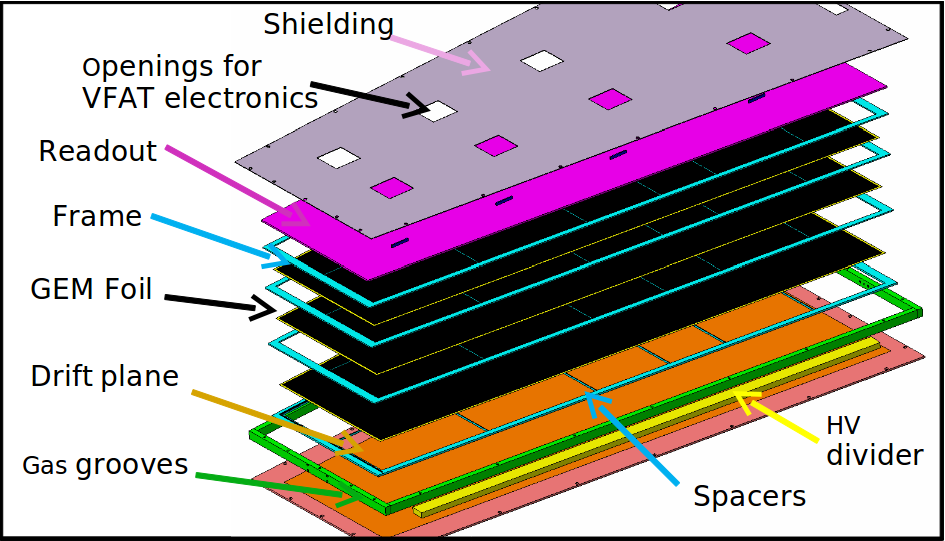
\includegraphics[width=0.95\textwidth]{figures/GEM/ge11cad.png}
		\caption{Layer by layer view of GEM detector}
		\label{fig:ge11}
	\end{center}
\end{figure} 
The trapezoidal chambers are sectored in $\eta$ partitions to cover $10^0$ each in the azimuthal sector and provide radial readout strip with the strip pointing to the LHC beam pipe (Figure \ref{fig:gemTrapezoidal}). In this design, the strip pitch varies from 0.6 mm (lower side) to 1.2 mm (upper side) with 8-$\eta$ sectors. To improve tracking capabilities, two GEM chambers will be mounted face-to-face to form a double layer called ``Super-Chamber". Thus each Super-Chamber will provide two impact points for each muon track. The gas gap configuration is: 3 mm (drift), 1 mm (transfer1), 2 mm(transfer2), and 1 mm (induction) as shown in Figure \ref{fig:tripple-gem}, which proved to be optimal for timing purposes. The gas mixture is $Ar/CO_2/CF_4~45/15/40$.
\begin{figure}[!htbp]
	\begin{center}
		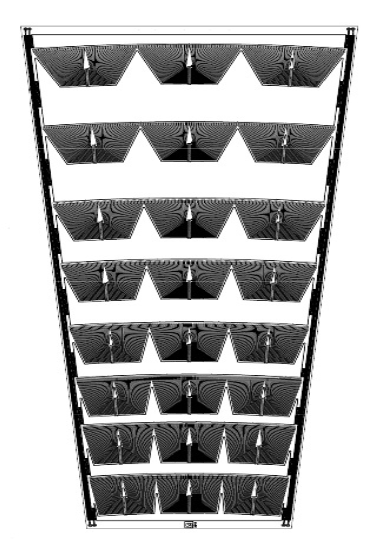
\includegraphics[width=0.55\textwidth]{figures/GEM/gemTrapezoidal.png}
		\caption{Drawing of a large trapezoidal CMS GEM chamber showing $8-\eta$ partitions, each}
		\label{fig:gemTrapezoidal}
	\end{center}
\end{figure} 
\begin{figure}[!htbp]
	\begin{center}
		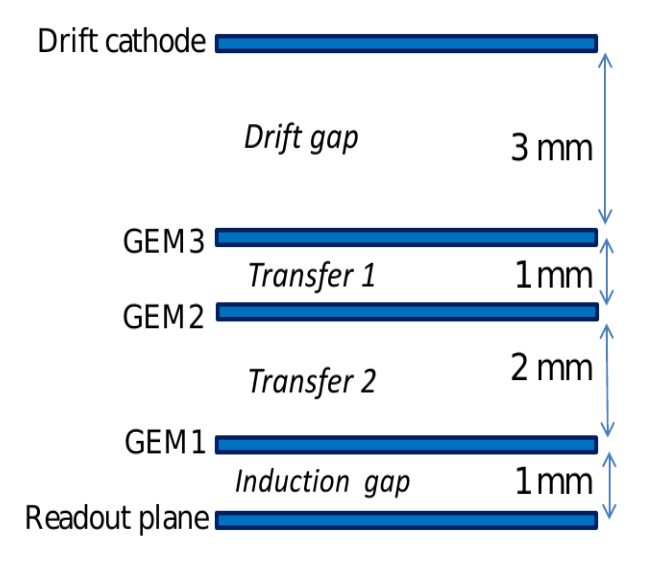
\includegraphics[width=0.65\textwidth]{figures/GEM/tripple-gem.png}
		\caption{Cross-section of the proposed triple-GEM showing the dimensions of the different gaps}
		\label{fig:tripple-gem}
	\end{center}
\end{figure} 
%The GEM production was achieved with the so called "Single-Mask" 
%\subsection{Test beam results}

Two large scale GEM chambers were tested at the SPS H2 beam line at CERN with 150GeV muon/pion beams. A hodoscope of small-area $(10\times 10 cm^2$) double sided GEM chambers was used to predict the hit position in the test chambers (Figure \ref{fig:tbsetup}). Each tracking chamber has, on each side, 256 readout strips with a pitch of 0.4 mm.

\begin{figure}[!htbp]
	\begin{center}
		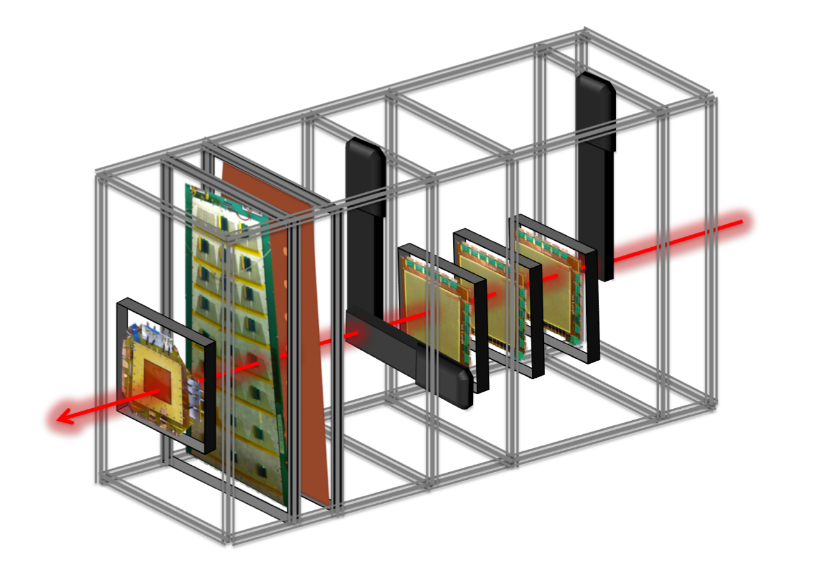
\includegraphics[width=0.95\textwidth]{figures/GEM/tbsetup.png}
		\caption{Schematic view of the test beam set-up with the three square GEM hodoscope and the trapezoidal CMS GEM chambers}
		\label{fig:tbsetup}
	\end{center}
\end{figure} 

The full scale CMS GEM chamber has a trapezoidal shape with dimensions of $990\times (220-445)mm$. The strips are segmented in $8-\eta$ partitions. Each partition is sectored along the $\phi$-coordinate into 3 readout sectors each with 128 strips. Thus 3072 channels are readout for the whole test chamber. During the test beam, two readout scenarios were used: digital TURBO/VFAT2 and Scalable Readout System (SRS) developed by RD51 collaboration and based on APV25 chips. The high voltage powering was realized using a ceramic high voltage divider. The CMS test chamber were placed, closed to the tracking hodoscope, on a vertically movable support to allow scanning. 

%Figure shows teh efficiency obtained


% chapter gas_electron_multiplier (end)